\let\tilde\widetilde
\def\SS{{\mathbb S}}
\def\X{{\mathbb X}}
%\def\bb{\mbox{\boldmath$b$}}
\def\bb{b}
\def\noisesd{\sigma}
\def\C{{\mathcal C}}
\def\A{{\mathcal A}}
\def\bigbracket#1#2#3{
\left[ 
\mbox{\begin{minipage}{#1}{
\vskip#2
#3
\vskip#2
\mbox{\ }
}\end{minipage}}
\right]
}

\msection{Data Representation (Objective 2)}
\label{sec:aim2}

The brain stores the same information in several ways across regions, 
each emphasizing different dimensions
of the input. In doing so, different features become accessible to the 
computations implemented in these regions. More
generally, by representing information in different ways, similar
learning rules automatically aggregate experience along
different dimensions and thereby extract complementary
knowledge. This can be contrasted with machine learning, both by the
simple fact that data are stored on disk in one format and that
finding relevant dimensions is often the output of the learning
algorithm rather a natural consequence of how the input is structured.
We will develop algorithms for machine representation of data that are
informed by our understanding of how the brain represents information
in different systems and leverage developments in embedding algorithms
in machine learning for advanced processing of fMRI data.

\biobackground{} Multiple brain systems represent inputs from the
world and store this information in different memory registers.
Although these representations are sometimes redundant (e.g., across
hemispheres in the same brain system), they often emphasize different
aspects of the input that are extracted via different neural pathways
or as a result of transformations across brain regions. In visual
cortex, for example, inputs with similar appearance (e.g.,
faces of siblings, Grand Canyon from different vistas, bananas
in a grocery store, etc.) will be stored together. In frontotemporal
cortex, inputs with the same conceptual or
functional meaning will be stored together despite differences in
appearance (e.g., pieces of clothing, cooking utensils, animals in the
ocean, etc.). In the ventral striatum and orbitofrontal cortex,
inputs with the same reward value will be represented
similarly irrespective of appearance or meaning (although subjective,
e.g., a favorite t-shirt and a nostalgic meal, an art show and a music
performance). Finally, in the hippocampus, overlap in appearance,
meaning, and reward can be discounted in favor of representing inputs
that co-occur over space or time together (e.g., a sequence of
landmarks on a commute, the people in a social group, events on a
memorable date, etc.). Different dimensions organize and
dominate representations in other brain systems, such as emotion,
modality, tasks, and motor actions. Here we will focus on
visual cortex and the hippocampus, two brain systems with mature
theories that address the nature of their representations.

After the retina and subcortical structures, the
human visual system is a hierarchy of cortical areas
starting from the first (V1) in the calcarine sulcus of
the occipital lobe~\citep{Felleman:1991}. There are four key
organizing principles from there. First, the visual areas in each
hemisphere receive input from the space contralateral to where the
eyes are fixated (i.e., retinotopic), with the input from a given side
of space projecting to both eyes converging in ocular dominance
columns in V1. Second, the areas are arrayed into at least two
streams~\citep{Mishkin:1983,Goodale:1992}: the ventral stream passing
on the inferior surface into the temporal lobe with areas coding for
the contralateral upper quadrant (V1-V3) and then the contralateral
upper and lower quadrants (V4 and beyond) involved in recognizing the identity of
objects~\citep{Arcaro:2009}; and the dorsal stream passing on the superior
surface into the parietal then frontal lobes with areas coding for the
contralateral lower quadrant (V1-V3) and upper and lower quadrants (V3a and beyond)
involved in processing object location and
action~\citep{Konen:2008}. Third, the visual areas in each stream
represent stimulus dimensions of increasing complexity:
from edges in V1, to color and texture in V4, to shape in ventral
occipital cortex, to object identity/category in inferior temporal (IT)
cortex~\citep{Grill-Spector:2003,Rousselet:2004}. Finally, paired with
increasing complexity is greater flexibility or ``tolerance'' to
variation in basic features, in terms of neurons in higher
areas covering larger areas of space (i.e., receptive fields) and having 
invariant neural representations (e.g., in IT, to size, position, viewpoint, etc.)~\citep{Rust:2010}.
These properties parallel those of deep convolutional neural networks
for object and scene recognition~\citep{Kriegeskorte:2015}. In
fact, optimizing the architecture of a deep net for object
recognition, without consideration of brain data, naturally
results in a model that predicts neuronal responses in visual
cortex~\citep{Yamins:2016}. The visual system is thus one of the best
understood brain systems and also the one that has had the
greatest impact to date on machine learning.

\setlength{\columnsep}{20pt}
\begin{wrapfigure}{R}{0.45\textwidth}
\centering
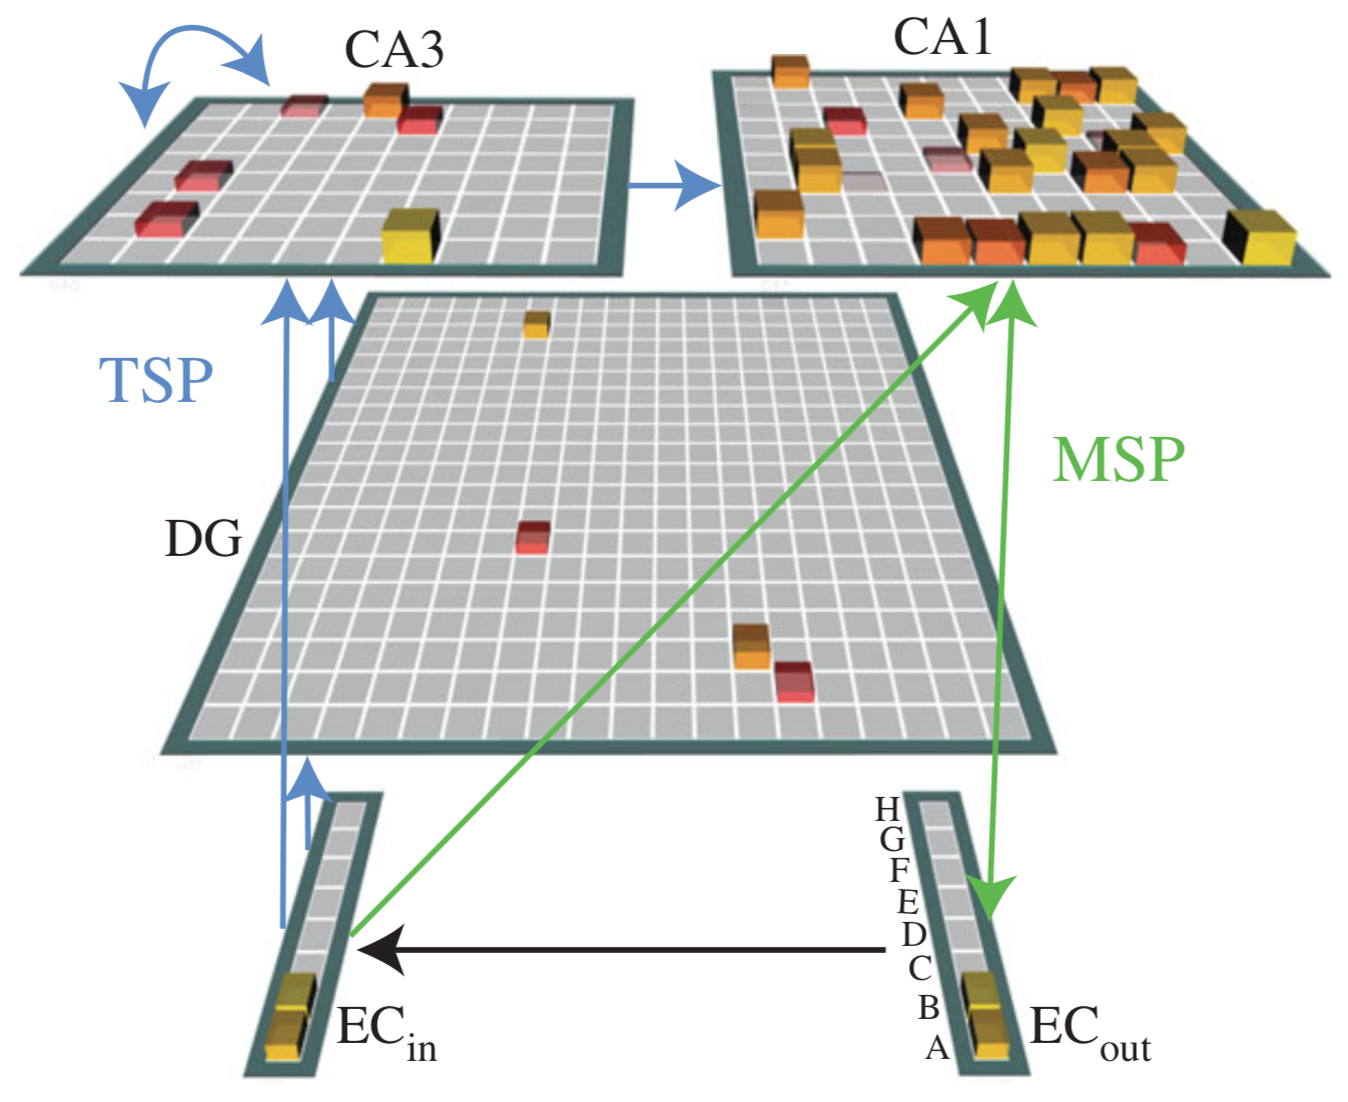
\includegraphics[width=.44\textwidth]{figs/hipp-model}
\caption{\small Biologically plausible neural network model of the
hippocampus. The network is trained to reproduce the pattern of
activity in the input (EC\textsubscript{in}) on the output
(EC\textsubscript{out}). Three hidden layers (DG, CA3, and CA1) learn
representations to support this mapping, with activity flow governed
by projections indicated by arrows. The TSP (blue
arrows) supports encoding into episodic memory via pattern separation
in DG and CA3 and retrieval via pattern completion within CA3. The
MSP (green arrows) supports statistical learning of
regularities across episodes. The height/yellowness of a unit both
reflect its activity level. From ~\citet{Schapiro:2017}.}
    \label{fig:hipp}
    \vskip-10pt
\end{wrapfigure}

Most models of the ventral stream treat IT as top of
the hierarchy~\citep[cf.][]{Saksida:2010}. However, IT is heavily interconnected with
the next most anterior areas, perirhinal cortex (PRC) and
parahippocampal cortex (PHC), which show selectivity for
objects and scenes,
respectively~\citep{Barense:2010,Davachi:2006,Ranganath:2012}. The PRC
and PHC project to the entorhinal cortex (ERC). The ERC in turn
provides input to the hippocampus, the structure critical for storing
long-term memories~\citep{Squire:1992}. Within the hippocampus, there
are four key subfields: dentate gyrus (DG), CA3, CA1, and
subiculum~\citep{Deng:2010,Shohamy:2013}. They are
connected via two pathways: the trisynaptic pathway (TSP) from ERC
to DG, CA3, and CA1; and the monosynaptic pathway (MSP) from ERC to
CA1~\citep{Schapiro:2017}. The hippocampus has two sources of
recurrence that allow it to bridge over time: locally within CA3 and
as a result of CA1 output to ERC that re-enters as
input~\citep{Kumaran:2016}. The function of the TSP is to
memorize specific input patterns, supporting ``episodic''
memory for individual moments in space and time (e.g., where I parked
my car this morning). This poses two challenges: (1) the
patterns need to be learned ``one-shot'' in that we never experience
the exact same episode twice, and (2) it is critical to avoid interference
from related memories (e.g., where I parked my car yesterday). The TSP
solves these challenges with \textit{pattern
separation}~\citep{Leutgeb:2007,Yassa:2011,Rolls:2016}: large capacity,
strong inhibition, and partial connectivity in DG and CA3 lead to
sparse, orthogonal representations of even highly overlapping ERC
inputs. The resulting memories are complex, unfurling over space and
time in different modalities, and these
components are linked via the auto-associative connections in
CA3~\citep{Wallenstein:1998}. By discounting feature overlap across
episodes and binding arbitrary features within episodes,
spatiotemporal co-occurrence dominates hippocampal representation.
Whereas theoretical models of the hippocampus from the connectionist
tradition have been around a long time and employ multi-layer
networks~\citep{McClelland:1995,Norman:2003}, the computational
properties of the hippocampus (e.g., pattern separation, learning rules and rates, 
bridging over time, relational binding, etc.) are not mainstream in machine learning.

\statbackground{}
Data representation algorithms are an important ingredient in contemporary
machine learning. One type, called embeddings, are used to represent
categorical data---for example, words in a natural language text---as
dense, high-dimensional ($d\approx 500$) vectors in Euclidean space \citep{Mikolov:2013}.
Embedding algorithms give representations well suited for downstream
algorithms. Sometimes they are learned in the first layer of
a deep neural network ~\citep{Bengio:2003}.  

Embeddings can be useful for many data types. For example, the popular
music entertainment site Spotify constructs embeddings of songs from
millions of user playlists, and uses these as the basis for
recommending new songs.  (``If you liked song $x\in\reals^{500}$,
perhaps you'll like the nearby song $x'\in\reals^{500}$.'')  This
machine learning based system eclipsed Pandora, which was based on a
hand-constructed representation, the ``music genome.'' Yet current
embedding algorithms such as the popular \texttt{word2vec} algorithm
are based on little more than a low-rank approximation (PCA) of simple
co-occurrence statistics.

Embeddings algorithms become more flexible when they are based
on statistical models, for instance using exponential family
models \citep{Rudolph:2016b,spherical}.
Consider a corpus of language $\mbx = \{x_1, \ldots, x_n\}$, where
each $x_i$ is a word from a vocabulary of terms. An exponential family
embedding has three components: (a) a notion of context for
each data point, e.g., a window of observed words around each word (b)
a form of the conditional distribution, e.g., for text a
categorical distribution over $V$ items is appropriate and (c) an
embedding structure that describes how parameters are shared
across data, e.g., for text one may assume that each term (such as
``walnut'' or ``bicycle'') shares the same representations wherever it
appears in the collection.
An exponential family embedding
posits two $d$-dimensional latent representations for each term $v$,
one is the embedding vector $\rho_v$ and the other is the
context vector $\alpha_v$, where $d$ is a hyperparameter.  The
model asserts that each observation is drawn from a conditional
distribution given its context. 
Exponential family embeddings generalize many existing methods for
learning distributed representations, including 
many variants of word2vec~\citep{Mikolov:2013}.  


\setlength{\columnsep}{20pt}
\begin{wrapfigure}{R}{0.45\textwidth}
\centering
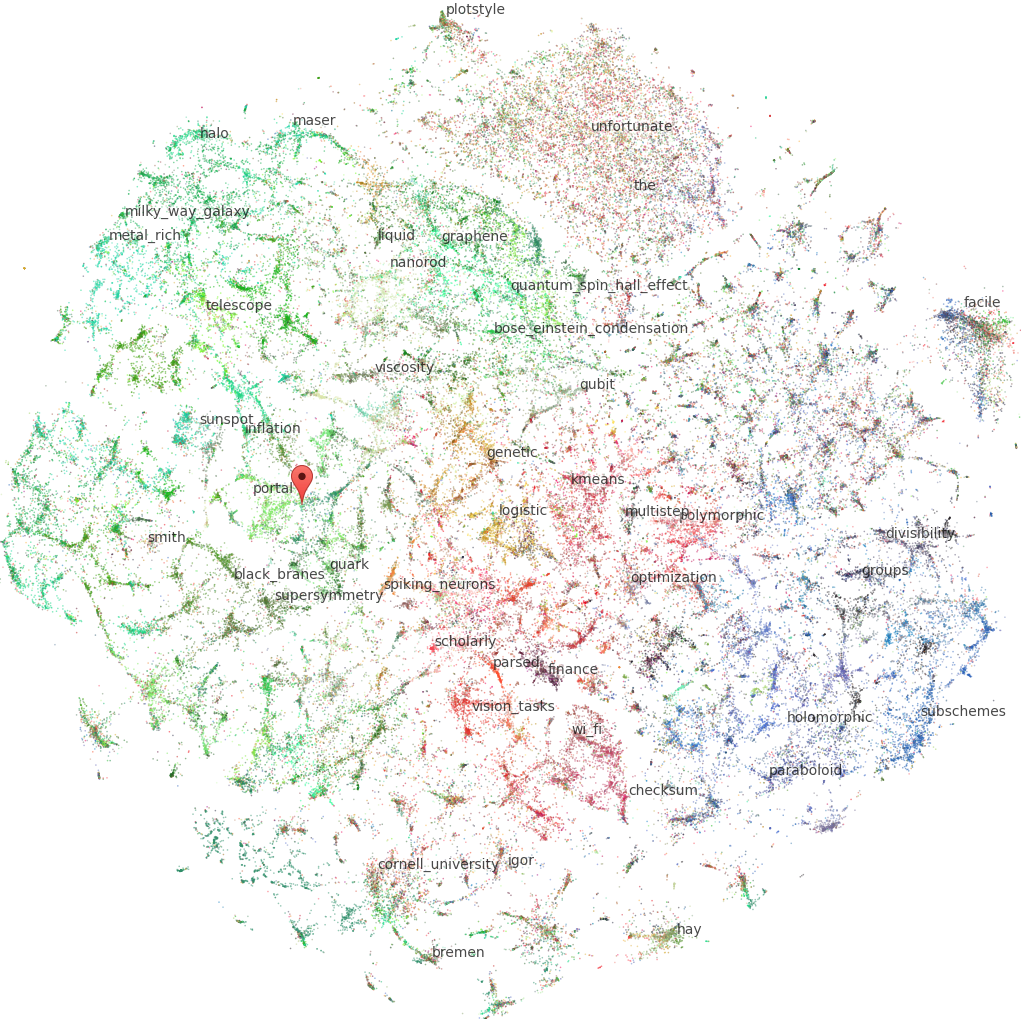
\includegraphics[width=.44\textwidth]{figs/ginsparg}
\caption{\small Embeddings of words appearing in scientific articles
posted on arXiv, mapped from 200 to two dimensions using
t-SNE \citep{ginsparg}. Constructed using only three months of
arXiv articles, for a 130,000 word vocabulary---using more data
leads to better embeddings.
Interactive exploration of the embeddings
using a Google maps interface: \href{http://www.cs.cornell.edu/~ginsparg/arxiv/gmaps2.html}{cs.cornell.edu/~ginsparg/arxiv/gmaps2.html}.
}
    \label{fig:arxiv}
    \vskip2pt
\end{wrapfigure}

Fitting such models is difficult, and requires robust methods for
computation and evaluation.  Variational inference approximates the
posterior by fitting a family of distributions over the latent
variables to be close in Kullback-Leibler
divergence~\citep{Jordan:1999,Blei:2017}.  In the case of embeddings,
the variational distribution is $q(\alpha_{1:V}, \rho_{1:V} ; \nu)$
and we fit the variational parameters $\nu$ to be close in KL
divergence to $p(\alpha_{1:V}, \rho_{1:V} \g \mbx)$.  Recent
innovations in black box variational inference~\citep{Ranganath:2014},
probabilistic programming~\citep{Kucukelbir:2017,Tran:2017}, and
variational autoencoders
\citep{kingma} as implemented, for example, in Google TensorFlow, allow us to do this generically and
scalably, easily fitting many types of models to large
data sets.  This enables the exploration of many variants of the
models, e.g., different types of contexts, different values of $d$,
and different underlying conditional distributions. We will use
this framework to develop more advanced and useful embedding
algorithms, inspired by current knowledge of higher-level cognition.


\project{Representations beyond co-occurrence statistics}
Distributed embedding representations in machine learning are almost
always based on co-occurrence statistics. For instance, when
constructing embeddings for words in text, names of colors (``red,''
``blue''...) will be nearby because they
tend to be used together. How can a richer knowledge of representation
in the brain inspire algorithms for processing text,
images, and audio? As discussed above, brain systems 
``embed'' in different ways, for example: visual cortex/appearance, frontotemporal
cortex/concepts, ventral striatum/reward, hippocampus/co-occurrence.
We will explore a wide variety of new machine learning models 
for representing data, using brain function as inspiration
for coding different aspects of data. For instance,
one embedding component learned in a reinforcement learning
setting might correspond to processing in orbitofrontal cortext;
another embedding component based on semantic parsing of scenes might correspond to processing in
the frontotemporal cortex. 
%Steps in such directions, have
%rguably made in recent work \citep{replearn}. 
The framework of exponential family embeddings and variational
inference provide powerful tools for this investigation.

\project{Enriched models for fMRI data}
In the other direction, from machine learning to cognitive neuroscience,
latent variable models and exponential family embeddings
are promising tools for advanced fMRI analysis. In particular,
embedding models have been used to decode fMRI activity patterns while
human subjects viewed words~\citep{Mitchell:2008}, listened to
stories~\citep{Huth:2016}, and watched movies~\citep{Vodrahalli:2017},
but in all of these cases the embeddings were derived from word
co-occurrences in text. The resulting semantic features are mapped onto
voxel activity patterns, allowing for prediction of the semantic content
of the brain at test. To the extent that voxels do not
represent semantic information, however, their feature weights will
be low and they will not contribute to the reconstruction. By learning
multiple embeddings in the project above, such as for visual, semantic,
reward, and spatiotemporal features, we will better capture the richness
of brain function with these models and improve the ability to decode
the contents of mind from a public movie-watching dataset~\citep[as used
in][]{Vodrahalli:2017}.

\project{Time-dependent, multiscale representations}
As discussed above, known computational properties of the hippocampus
including pattern separation, different learning rates, and bridging
over time, have not yet entered the mainstream of machine learning.
We will study new learning architectures that attempt to mimic, even
if only as a computational metaphor, these capabilities in cognition.
To capture dependence on time, we will earlier work on dynamic topic
models~\citep{Blei:2006d}. Dynamic topic models capture how the
latent themes in a collection can grow and shrink and change over
time. By introducing multiple latent time series threads in such a
model, each having a different time scale, we can model different
learning rates. Dynamic topic models were
developed specifically for language.  We will generalize this idea to
capture the evolution of distributed representations over time. In
the exponential family embedding framework, this amounts to placing a
linear dynamic prior on the embedding vectors or the context vectors,
or both.
